
\begin{figure}[h]
    \centering
    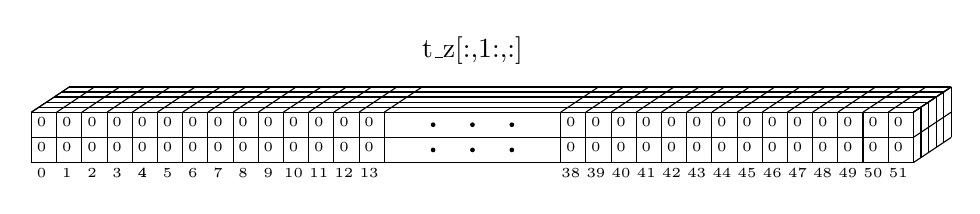
\begin{tikzpicture}
        % Define grid dimensions
        \def\n{2} % N = 2 rows (front face height)
        \def\m{35} % M = 20 columns (front face width)
        \def\depth{5} % Depth of the cube (z-axis, number of cells in depth)
        \def\cellsize{0.32} % Size of each cell

        % Define 3D perspective skew for top and right faces
        \def\skewx{0.3} % Skew factor for x-axis (right face)
        \def\skewy{0.2} % Skew factor for y-axis (top face)

        % --- Front Face (now a 2x20 grid) ---
        % Draw the grid - Horizontal lines
        \foreach \i in {0,...,\n} {
            \draw[black] (0,\i*\cellsize) -- (\m*\cellsize,\i*\cellsize); % Horizontal lines
        }
        % \foreach \j in {0,...,\m} {
        %     \draw[black] (\j*\cellsize,0) -- (\j*\cellsize,\n*\cellsize);
        %     }
        
        % Draw the grid - Vertical lines with condition
        \foreach \j in {0,...,\m} {
            \ifnum\j<15 % Check if j < 7
                \draw[black] (\j*\cellsize,0) -- (\j*\cellsize,\n*\cellsize); % Draw line
            \else
                \ifnum\j>20 % Check if j > 13
                    \draw[black] (\j*\cellsize,0) -- (\j*\cellsize,\n*\cellsize); % Draw line
                \fi
            \fi
        }

        % Add the shape label below the grid
        \node[above] at ({\m/2*\cellsize}, 3.5*\cellsize) {\pyvar{t\_z[:,1:,:]}};
    
        Place dots in the middle of the front face (e.g., in row 1, columns 9, 10, 11)
        \foreach \j in {0,1,2} {
            \fill[black] ({(1-\j)/2+\m*\cellsize/2}, 1*\cellsize-0.5*\cellsize) circle (0.03); % Dots in row 1 (y=0.5)
        }
                \foreach \j in {0,1,2} {
            \fill[black] ({(1-\j)/2+\m*\cellsize/2}, 1*\cellsize+0.5*\cellsize) circle (0.03); % Dots in row 1 (y=0.5)
        }

        % Draw the outer rectangle for the front face
        \draw[black] (0,0) rectangle (\m*\cellsize, \n*\cellsize);



        \node at (0.4*\cellsize, \n*\cellsize-0.4*\cellsize) {\tiny 0};
        \node at (0.4*\cellsize, \n*\cellsize-1.4*\cellsize) {\tiny 0};
        
        \node at (1.4*\cellsize, \n*\cellsize-0.4*\cellsize) {\tiny 0};
        \node at (1.4*\cellsize, \n*\cellsize-1.4*\cellsize) {\tiny 0};

        \node at (2.4*\cellsize, \n*\cellsize-0.4*\cellsize) {\tiny 0};
        \node at (2.4*\cellsize, \n*\cellsize-1.4*\cellsize) {\tiny 0};

        \node at (3.4*\cellsize, \n*\cellsize-0.4*\cellsize) {\tiny 0};
        \node at (3.4*\cellsize, \n*\cellsize-1.4*\cellsize) {\tiny 0};

        \node at (4.4*\cellsize, \n*\cellsize-0.4*\cellsize) {\tiny 0};
        \node at (4.4*\cellsize, \n*\cellsize-1.4*\cellsize) {\tiny 0};
        
        \node at (5.4*\cellsize, \n*\cellsize-0.4*\cellsize) {\tiny 0};
        \node at (5.4*\cellsize, \n*\cellsize-1.4*\cellsize) {\tiny 0};
        
        \node at (6.4*\cellsize, \n*\cellsize-0.4*\cellsize) {\tiny 0};
        \node at (6.4*\cellsize, \n*\cellsize-1.4*\cellsize) {\tiny 0};
        
        \node at (7.4*\cellsize, \n*\cellsize-0.4*\cellsize) {\tiny 0};
        \node at (7.4*\cellsize, \n*\cellsize-1.4*\cellsize) {\tiny 0};
        
        \node at (8.4*\cellsize, \n*\cellsize-0.4*\cellsize) {\tiny 0};
        \node at (8.4*\cellsize, \n*\cellsize-1.4*\cellsize) {\tiny 0};
        
        \node at (9.4*\cellsize, \n*\cellsize-0.4*\cellsize) {\tiny 0};
        \node at (9.4*\cellsize, \n*\cellsize-1.4*\cellsize) {\tiny 0};
        
        \node at (10.4*\cellsize, \n*\cellsize-0.4*\cellsize) {\tiny 0};
        \node at (10.4*\cellsize, \n*\cellsize-1.4*\cellsize) {\tiny 0};
        
        \node at (11.4*\cellsize, \n*\cellsize-0.4*\cellsize) {\tiny 0};
        \node at (11.4*\cellsize, \n*\cellsize-1.4*\cellsize) {\tiny 0};
        
        \node at (12.4*\cellsize, \n*\cellsize-0.4*\cellsize) {\tiny 0};
        \node at (12.4*\cellsize, \n*\cellsize-1.4*\cellsize) {\tiny 0};

        \node at (13.4*\cellsize, \n*\cellsize-0.4*\cellsize) {\tiny 0};
        \node at (13.4*\cellsize, \n*\cellsize-1.4*\cellsize) {\tiny 0};

    %%% RIGHT HAND SIDE
        \node at (21.4*\cellsize, \n*\cellsize-0.4*\cellsize) {\tiny 0};
        \node at (21.4*\cellsize, \n*\cellsize-1.4*\cellsize) {\tiny 0};
        
        \node at (22.4*\cellsize, \n*\cellsize-0.4*\cellsize) {\tiny 0};
        \node at (22.4*\cellsize, \n*\cellsize-1.4*\cellsize) {\tiny 0};

        \node at (23.4*\cellsize, \n*\cellsize-0.4*\cellsize) {\tiny 0};
        \node at (23.4*\cellsize, \n*\cellsize-1.4*\cellsize) {\tiny 0};

        \node at (24.4*\cellsize, \n*\cellsize-0.4*\cellsize) {\tiny 0};
        \node at (24.4*\cellsize, \n*\cellsize-1.4*\cellsize) {\tiny 0};

        \node at (25.4*\cellsize, \n*\cellsize-0.4*\cellsize) {\tiny 0};
        \node at (25.4*\cellsize, \n*\cellsize-1.4*\cellsize) {\tiny 0};
        
        \node at (26.4*\cellsize, \n*\cellsize-0.4*\cellsize) {\tiny 0};
        \node at (26.4*\cellsize, \n*\cellsize-1.4*\cellsize) {\tiny 0};
        
        \node at (27.4*\cellsize, \n*\cellsize-0.4*\cellsize) {\tiny 0};
        \node at (27.4*\cellsize, \n*\cellsize-1.4*\cellsize) {\tiny 0};
        
        \node at (28.4*\cellsize, \n*\cellsize-0.4*\cellsize) {\tiny 0};
        \node at (28.4*\cellsize, \n*\cellsize-1.4*\cellsize) {\tiny 0};
        
        \node at (29.4*\cellsize, \n*\cellsize-0.4*\cellsize) {\tiny 0};
        \node at (29.4*\cellsize, \n*\cellsize-1.4*\cellsize) {\tiny 0};
        
        \node at (30.4*\cellsize, \n*\cellsize-0.4*\cellsize) {\tiny 0};
        \node at (30.4*\cellsize, \n*\cellsize-1.4*\cellsize) {\tiny 0};
        
        \node at (31.4*\cellsize, \n*\cellsize-0.4*\cellsize) {\tiny 0};
        \node at (31.4*\cellsize, \n*\cellsize-1.4*\cellsize) {\tiny 0};
        
        \node at (32.4*\cellsize, \n*\cellsize-0.4*\cellsize) {\tiny 0};
        \node at (32.4*\cellsize, \n*\cellsize-1.4*\cellsize) {\tiny 0};
        
        \node at (33.4*\cellsize, \n*\cellsize-0.4*\cellsize) {\tiny 0};
        \node at (33.4*\cellsize, \n*\cellsize-1.4*\cellsize) {\tiny 0};

        \node at (34.4*\cellsize, \n*\cellsize-0.4*\cellsize) {\tiny 0};
        \node at (34.4*\cellsize, \n*\cellsize-1.4*\cellsize) {\tiny 0};


        % Place numbers in the front face (row 1, i.e., y=\n*\cellsize-1.4*\cellsize)
        % Let's use different numbers to distinguish the rows

        % \node at (16.4*\cellsize, \n*\cellsize-1.4*\cellsize) {\tiny 0};
        % \node at (17.4*\cellsize, \n*\cellsize-1.4*\cellsize) {\tiny 2};
        % \node at (18.4*\cellsize, \n*\cellsize-1.4*\cellsize) {\tiny 1};
        % \node at (19.4*\cellsize, \n*\cellsize-1.4*\cellsize) {\tiny 0};

        % --- Top Face ---
        % Draw the top face as a parallelogram
        \draw[black] (\m*\cellsize, \n*\cellsize) -- ++(\depth*\cellsize*\skewx, \depth*\cellsize*\skewy); % Right edge of top face
        \draw[black] (0, \n*\cellsize) -- ++(\depth*\cellsize*\skewx, \depth*\cellsize*\skewy); % Left edge of top face
        \draw[black] (\m*\cellsize, \n*\cellsize) -- (0, \n*\cellsize); % Front edge (already drawn)
        \draw[black] (\m*\cellsize+\depth*\cellsize*\skewx, \n*\cellsize+\depth*\cellsize*\skewy) -- (0+\depth*\cellsize*\skewx, \n*\cellsize+\depth*\cellsize*\skewy); % Back edge

                % % Draw grid lines on the top face (along x-axis)
        \foreach \j in {0,...,\m} {
            \ifnum\j<15 % Same condition as front face
                \draw[black] (\j*\cellsize, \n*\cellsize) -- ++(\depth*\cellsize*\skewx, \depth*\cellsize*\skewy);
            \else
                \ifnum\j>20
                    \draw[black] (\j*\cellsize, \n*\cellsize) -- ++(\depth*\cellsize*\skewx, \depth*\cellsize*\skewy);
                \fi
            \fi
        }

        % % Draw grid lines on the top face (along x-axis)
        % \foreach \j in {0,...,\m} {
        %     \ifnum\j<7 % Same condition as front face
        %         \draw[black] (\j*\cellsize, \n*\cellsize) -- ++(\depth*\cellsize*\skewx, \depth*\cellsize*\skewy);
        %     \else
        %         \ifnum\j>13
        %             \draw[black] (\j*\cellsize, \n*\cellsize) -- ++(\depth*\cellsize*\skewx, \depth*\cellsize*\skewy);
        %         \fi
        %     \fi
        % }

        % Draw grid lines on the top face (along z-axis, depth)
        \foreach \k in {0,...,\depth} {
            \draw[black] (\m*\cellsize+\k*\cellsize*\skewx, \n*\cellsize+\k*\cellsize*\skewy) -- (0+\k*\cellsize*\skewx, \n*\cellsize+\k*\cellsize*\skewy);
        }

        % --- Right Face ---
        % % Draw the right face as a parallelogram
        % \draw[black] (\m*\cellsize, \n*\cellsize) -- ++(\depth*\cellsize*\skewx, -\depth*\cellsize*\skewy); % Top edge of right face
        % \draw[black] (\m*\cellsize, 0) -- ++(\depth*\cellsize*\skewx, -\depth*\cellsize*\skewy); % Bottom edge of right face
        % \draw[black] (\m*\cellsize, \n*\cellsize) -- (\m*\cellsize, 0); % Front edge (already drawn)
        % \draw[black] (\m*\cellsize+\depth*\cellsize*\skewx, \n*\cellsize-\depth*\cellsize*\skewy) -- (\m*\cellsize+\depth*\cellsize*\skewx, -\depth*\cellsize*\skewy); % Back edge

        % Draw grid lines on the right face (along y-axis, height)
        \foreach \i in {0,...,\n} {
            \draw[black] (\m*\cellsize, \i*\cellsize) -- ++(\depth*\cellsize*\skewx, \depth*\cellsize*\skewy);
        }

        % Draw grid lines on the right face (along z-axis, depth)
        \foreach \k in {0,...,\depth} {
            \draw[black] (\m*\cellsize+\k*\cellsize*\skewx, \n*\cellsize+\k*\cellsize*\skewy) -- (\m*\cellsize+\k*\cellsize*\skewx, 0+\k*\cellsize*\skewy);
        }

    \node at (0.4*\cellsize, \n*\cellsize-2.4*\cellsize) {\tiny 0};
    \node at (1.4*\cellsize, \n*\cellsize-2.4*\cellsize) {\tiny 1};
    \node at (2.4*\cellsize, \n*\cellsize-2.4*\cellsize) {\tiny 2};
    \node at (3.4*\cellsize, \n*\cellsize-2.4*\cellsize) {\tiny 3};
    \node at (4.4*\cellsize, \n*\cellsize-2.4*\cellsize) {\tiny 4};
    \node at (4.4*\cellsize, \n*\cellsize-2.4*\cellsize) {\tiny 4};
    \node at (5  .4*\cellsize, \n*\cellsize-2.4*\cellsize) {\tiny 5};
    \node at (6.4*\cellsize, \n*\cellsize-2.4*\cellsize) {\tiny 6};
    \node at (7.4*\cellsize, \n*\cellsize-2.4*\cellsize) {\tiny 7};
    \node at (8.4*\cellsize, \n*\cellsize-2.4*\cellsize) {\tiny 8};
    \node at (9.4*\cellsize, \n*\cellsize-2.4*\cellsize) {\tiny 9};
    \node at (10.4*\cellsize, \n*\cellsize-2.4*\cellsize) {\tiny 10};
    \node at (11.4*\cellsize, \n*\cellsize-2.4*\cellsize) {\tiny 11};
    \node at (12.4*\cellsize, \n*\cellsize-2.4*\cellsize) {\tiny 12};
    \node at (13.4*\cellsize, \n*\cellsize-2.4*\cellsize) {\tiny 13};

    \node at (21.4*\cellsize, \n*\cellsize-2.4*\cellsize) {\tiny 38};
    \node at (22.4*\cellsize, \n*\cellsize-2.4*\cellsize) {\tiny 39};
    \node at (23.4*\cellsize, \n*\cellsize-2.4*\cellsize) {\tiny 40};
    \node at (24.4*\cellsize, \n*\cellsize-2.4*\cellsize) {\tiny 41};
    \node at (25.4*\cellsize, \n*\cellsize-2.4*\cellsize) {\tiny 42};
    \node at (26.4*\cellsize, \n*\cellsize-2.4*\cellsize) {\tiny 43};
    \node at (27.4*\cellsize, \n*\cellsize-2.4*\cellsize) {\tiny 44};
    \node at (28.4*\cellsize, \n*\cellsize-2.4*\cellsize) {\tiny 45};
    \node at (29.4*\cellsize, \n*\cellsize-2.4*\cellsize) {\tiny 46};
    \node at (30.4*\cellsize, \n*\cellsize-2.4*\cellsize) {\tiny 47};
    \node at (31.4*\cellsize, \n*\cellsize-2.4*\cellsize) {\tiny 48};
    \node at (32.4*\cellsize, \n*\cellsize-2.4*\cellsize) {\tiny 49};
    \node at (33.4*\cellsize, \n*\cellsize-2.4*\cellsize) {\tiny 50};
    \node at (34.4*\cellsize, \n*\cellsize-2.4*\cellsize) {\tiny 51};
    
    \end{tikzpicture}
\caption{\small Tensor \pyvar{t\_z[:,1:,:]} represents player actions. The above tensor corresponds to sample game round from Table 1.}
    \label{fig:card_cube}
\end{figure}

% Reference the figure in the text

